\section{Market Model}

\begin{figure}[h!]
  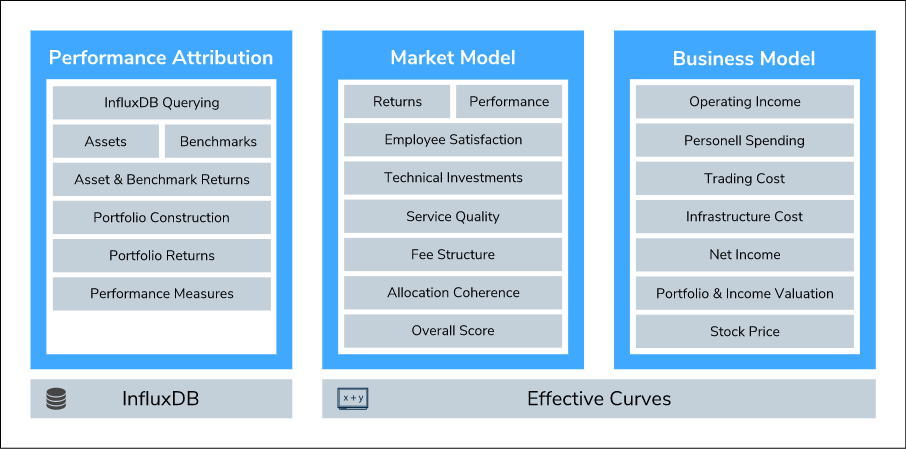
\includegraphics[width=\textwidth]{img/market_model.png}
  \caption{Market Model Overview}
  \centering
\end{figure}

The PFM-Game market model is a module that produces period results based on the business decisions and portfolio allocations of teams participating in a given game. The market model is separated into several subcomponents that, when applied in sequence, produce results for a period of the game.

\subsection{Data and Data Ingestion}
The underlying data driving all portfolio-related calculations in the market model is comprised of several hunderd time-series that are stored in InfluxDB. The majority of these time-series describe asset price or return indices (i.e., asset prices normalized by the payment of dividends and other interest) as extracted from the Thomson Reuters Datastream platform. Further relevant time-series are based on macroeconomic data extracted from the FRED (Federal Reserve Economic Data) database. These data are used to calculate portfolio and benchmark returns as well as parameters of an economic forecast.

The above described data can be extracted from Datastream and FRED and ingested into an instance of InfluxDB automatically by means of a Python module that was created as an extension to the PFM-Simulation project. Data to be ingested is defined inside an assets.csv file in the following CSV format:

\begin{table}[h!]
  \begin{tabular}{lllllll}
    \toprule
    Name & Symbol  & Start Date & Market      & Data Type & Asset Type & Currency \\
    \midrule
    SWISS BOND AAA & SWBND3A & 29.12.2006 & Switzerland & RI        & BONDS      & CHF      \\
    NESTLE 'R'     & S:NESN  & 01.01.1973 & Switzerland & RI        & EQUITY     & CHF      \\
    \bottomrule
  \end{tabular}
  \centering
  \caption{Exemplary assets in a valid assets.csv definition format (optional columns omitted)}
\end{table}

During processing of the CSV definition of all assets, the module will incrementally extend existing time-series with new data up to the current day. Time-series that were not previously available will be stored as a new series in full-length.


\subsection{Performance Attribution}
The performance attribution module is the first module in the sequence of market model calculations that are applied to an incoming request.


\subsection{Market Model}



\subsection{Business Model}



\subsection{API Specification}
